\chapter{Resultados de la armonización}\label{cap:result}

\section{El nivel del factor importa}

La tabla~\ref{tab:niveles} compara los tres niveles del factor en los dos ejercicios. El factor por estado y mes con contracción reduce el error por estado y mes de $24.8\,\%$ a $12.9\,\%$ en el ejercicio de un año fuera, y de $21.3\,\%$ a $14.5\,\%$ en años no vistos: entre un tercio y la mitad menos error que con un factor único. El error anual nacional cae de $4.9\,\%$ a $1.3\,\%$ y de $3.3\,\%$ a $2.1\,\%$.

\begin{table}[H]
\centering
\caption{Error (WAPE, \%) por nivel del factor. «UF» es el ejercicio de un año fuera (2012--2019) y «NV», el de años no vistos (2020--2025).}\label{tab:niveles}
\small
\begin{tabular}{@{}lrrrrrr@{}}
\toprule
 & \multicolumn{2}{c}{Estado y mes} & \multicolumn{2}{c}{Nacional y mes} & \multicolumn{2}{c}{Nacional y año}\\
\cmidrule(lr){2-3}\cmidrule(lr){4-5}\cmidrule(lr){6-7}
Factor & UF & NV & UF & NV & UF & NV \\
\midrule
Factor único (todo México, todo el año) & 24.8 & 21.3 & 10.4 & 8.2 & 4.9 & 3.3 \\
Factor por mes (nacional) & 22.9 & 21.2 & 6.3 & 6.9 & 4.6 & 4.0 \\
Factor por estado y mes (contracción $\tau$=100) & 12.9 & 14.5 & 3.7 & 5.4 & 1.3 & 2.1

\\
\bottomrule
\end{tabular}
\end{table}

\begin{figure}[H]
\centering
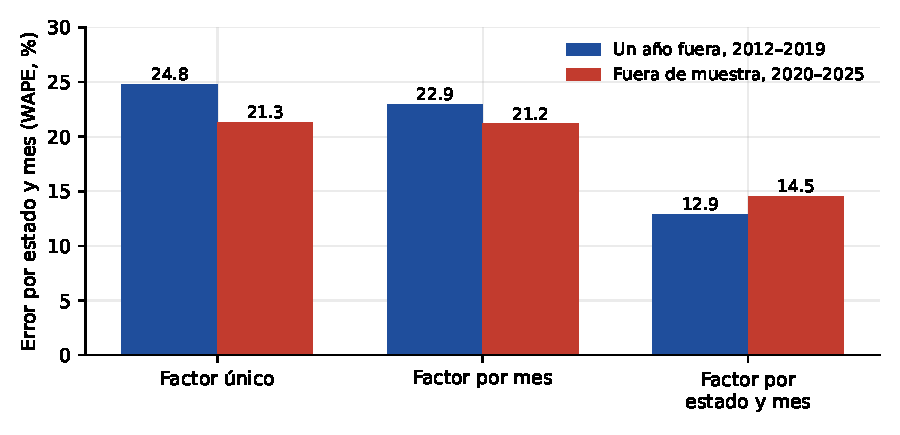
\includegraphics[width=0.85\textwidth]{fig/fig_niveles.pdf}
\caption{Error por estado y mes según el nivel del factor.}\label{fig:niveles}
\end{figure}

Hay dos lecturas distintas. El factor por mes (nacional) reduce mucho el error nacional por mes (de $10.4\,\%$ a $6.3\,\%$ en un año fuera) porque corrige la estacionalidad de la razón, pero apenas mejora el error por estado, porque no distingue entre estados. El factor por estado y mes corrige ambas cosas.

\begin{table}[H]
\centering
\caption{Sesgo relativo (\%) y correlación mensual nacional. UF: un año fuera; NV: años no vistos.}\label{tab:sesgo}
\small
\begin{tabular}{@{}lrrrr@{}}
\toprule
 & \multicolumn{2}{c}{Sesgo (\%)} & \multicolumn{2}{c}{Correlación mensual} \\
\cmidrule(lr){2-3}\cmidrule(lr){4-5}
Factor & UF & NV & UF & NV \\
\midrule
Factor único (todo México, todo el año) & $-$0.34 & $-$1.13 & 0.9921 & 0.9939 \\
Factor por mes (nacional) & $-$0.24 & $-$0.91 & 0.9990 & 0.9939 \\
Factor por estado y mes (contracción $\tau$=100) & $-$0.06 & 0.39 & 0.9993 & 0.9959

\\
\bottomrule
\end{tabular}
\end{table}

El sesgo de la serie armonizada es prácticamente cero: $-0.06\,\%$ en un año fuera y $+0.39\,\%$ en años no vistos para el factor elegido. Con los factores de 2012--2019, la suma 2013--2025 de VIIRS armonizado difiere de la de MODIS observado en solo \difArm{}\,\%. Ese número, ojo, \emph{no} es fuera de muestra: 2013--2019 pertenece al entrenamiento. Los ejercicios del capítulo anterior son los que valen para juzgar el método.

\section{Ideas sofisticadas que no ayudaron}

La tabla~\ref{tab:variantes} muestra las variantes de conteo de VIIRS. Fusionar los píxeles dentro de una huella de 1 km y filtrar por FRP son decisiones razonables, pero empeoran todas las métricas: el error anual fuera de muestra pasa de $2.1\,\%$ a entre $4.4\,\%$ y $7.6\,\%$ y aparece un sesgo negativo de hasta $-6.6\,\%$.

\begin{table}[H]
\centering
\caption{Variantes del conteo de VIIRS con factor por estado y mes. WAPE (\%) por estado y mes y anual nacional; sesgo en años no vistos. UF: un año fuera; NV: años no vistos.}\label{tab:variantes}
\small
\begin{tabular}{@{}lrrrrr@{}}
\toprule
 & \multicolumn{2}{c}{Estado y mes} & \multicolumn{2}{c}{Nacional y año} & Sesgo \\
\cmidrule(lr){2-3}\cmidrule(lr){4-5}\cmidrule(lr){6-6}
Variante & UF & NV & UF & NV & NV \\
\midrule
\textbf{Sin huella ni umbral de FRP (elegida)} & 12.9 & 14.5 & 1.3 & 2.1 & 0.4 \\
Con huella de 1 km (fusiona píxeles VIIRS) & 13.8 & 15.9 & 2.7 & 4.4 & $-$3.3 \\
Huella de 1 km $+$ FRP VIIRS $\geq$ 2 MW & 14.8 & 16.1 & 4.8 & 6.9 & $-$5.9 \\
Huella de 1 km $+$ FRP VIIRS $\geq$ 4 MW & 15.1 & 16.3 & 4.8 & 7.6 & $-$6.6 \\
Huella de 1 km $+$ FRP VIIRS $\geq$ 6 MW & 14.7 & 15.6 & 3.8 & 6.8 & $-$5.4

\\
\bottomrule
\end{tabular}
\end{table}

¿Por qué empeoran? Una explicación plausible, que no probamos por separado, es que la razón entre sensores se estima \emph{para el conteo que se usa}. Al recortar o fusionar, el conteo de VIIRS pierde fuegos que MODIS sí ve en proporciones que cambian entre años; el factor ya no es estable y la calibración no lo absorbe. El resultado que sí está medido es el comparativo: no ayudan, así que la solución simple gana.

\section{Terra a Terra más Aqua}\label{sec:val-terra}

Con la misma lógica de dejar un año fuera, dentro de 2003--2011, el factor de Terra a Terra más Aqua tiene un error de \terraSM{}\,\% por estado y mes, \terraNM{}\,\% nacional por mes y \terraAN{}\,\% anual, con sesgo $\terraSesgo\,\%$. Frente al factor de VIIRS en el mismo ejercicio ($12.9\,\%$, $3.7\,\%$ y $1.3\,\%$), el error por estado y mes es parecido y los errores nacionales son mayores. Y recuérdese que esta validación no puede probar que la relación se conserve en 2000--2002.

\section{La estacionalidad de las quemas}

Con la serie armonizada se ve con claridad la estacionalidad (figura~\ref{fig:estacionalidad}): abril y mayo concentran $65.7\,\%$ de los hotspots equivalentes (dos de cada tres) y marzo a junio, $83.7\,\%$ (años 2001 a 2025, con todos los hotspots equivalentes juntos). Es una descripción de la serie, no un resultado de la validación.

\begin{figure}[H]
\centering
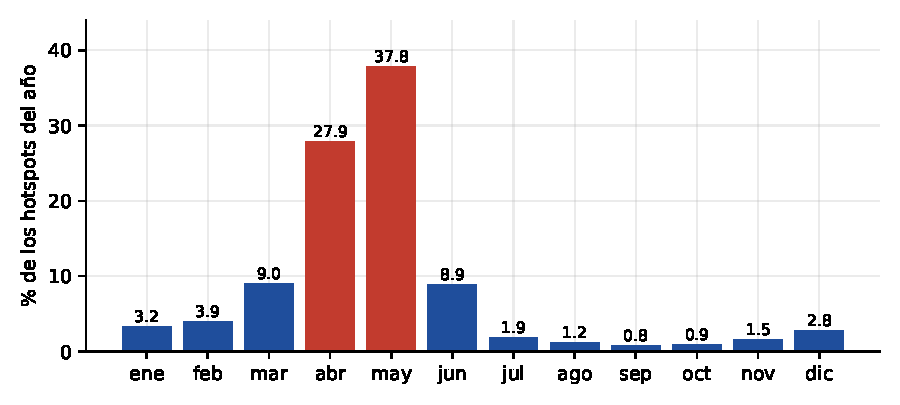
\includegraphics[width=0.85\textwidth]{fig/fig_estacionalidad.pdf}
\caption{Porcentaje de los hotspots equivalentes de cada mes, años 2001--2025 (todos los años juntos). En rojo, abril y mayo.}\label{fig:estacionalidad}
\end{figure}

\begin{ideaclave}[Idea clave del capítulo]
La serie armonizada reproduce a MODIS con error anual nacional de $1.3\,\%$ y $2.1\,\%$, y por estado y mes de $12.9\,\%$ y $14.5\,\%$. Calibrar por estado y mes reduce el error por estado y mes entre un tercio y la mitad frente a un factor único. Fusionar píxeles y filtrar por FRP, que parecían buenas ideas, empeoran el resultado.
\end{ideaclave}
